% $Header$

\documentclass{beamer}

% Copyright (c)  2021  HiKlas Ltd.
% Permission is granted to copy, distribute and/or modify this document
% under the terms of the GNU Free Documentation License, Version 1.3
% or any later version published by the Free Software Foundation;
% with no Invariant Sections, no Front-Cover Texts, and no Back-Cover Texts.
% A copy of the license is included in the section entitled "GNU
% Free Documentation License".
%
% Based on the Beamer generic-ornate-15min-45min.en.tex template by
% Till Tantau <tantau@users.sourceforge.net>



\mode<presentation>
{
  \usetheme{CambridgeUS}
}

\usepackage[english]{babel}
\usepackage[latin1]{inputenc}
\usepackage[T1]{fontenc}
% Or whatever. Note that the encoding and the font should match. If T1
% does not look nice, try deleting the line with the fontenc.

% These packages are used for drawing circuits
\usepackage{tikz}
\usepackage[siunitx,european,americanresistors]{circuitikz}


% Information about the presentation 
\title{Introduction to Machine Code}
\subtitle{Understanding Computer Internals}
\author{Fiona Bianchi}
\institute{HiKlas Ltd}
\date{August 2021}
\subject{Talks}
\pgfdeclareimage[height=0.5cm]{company-logo}{../assets/HiklasLogo.eps}
\logo{\pgfuseimage{company-logo}}

% Table of contents for each Subsection
\AtBeginSubsection[]
{
  \begin{frame}<beamer>{Outline}
    \tableofcontents[currentsection,currentsubsection]
  \end{frame}
}

% TODO: Nope, I don't think I want this put leaving it in just in case
% TODO: to remove when absolutely sure
% If you wish to uncover everything in a step-wise fashion, uncomment
% the following command: 
%\beamerdefaultoverlayspecification{<+->}


\begin{document}

\begin{frame}
  \titlepage
\end{frame}

\begin{frame}{Outline}
  \tableofcontents
  % TODO: What is "pausesections" for?
  % You might wish to add the option [pausesections]
\end{frame}


\section{Back to Basics}

\subsection[Switches]{Simple Electronics Switches}

\begin{frame}{A Light Switch}

  \begin{columns}
    \column{0.5\textwidth}
    \begin{itemize}
    \item
      The simplest electronic cicruit
    \item
      Switch has two positions, ``on'' or ``off''
    \item
      What has this got to do with computers?
    \end{itemize}

    \column{0.5\textwidth}
    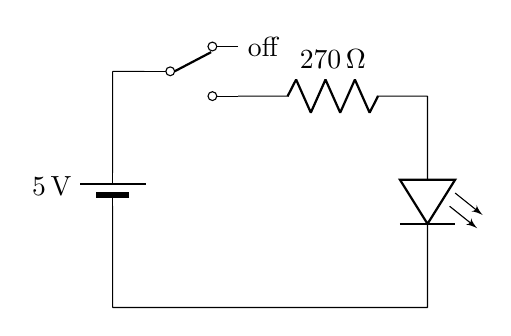
\begin{tikzpicture}
      \coordinate (as) at (4,3);
      \draw 
	(0, 3) to [battery2, l_=5<\volt>,] (0,0) 
	(1, 3) node[spdt] (Sw1) {}
	(0, 3) to [short] (Sw1.in)
		(Sw1.out 1) node[right] {off} 
	(Sw1.out 2) to [R,label=270<\ohm>] (as |- Sw1.out 2)
	(as |- Sw1.out 2) to [empty led] (4,0)
	(4,0) to (0,0);
    \end{tikzpicture}
  \end{columns}
\end{frame}

\begin{frame}{A Backwards Light Switch}

  \begin{columns}
    \column{0.5\textwidth}
    \begin{itemize}
    \item
      Someone wires a switch wrongly
    \item
      You have to flick it to ``off'' to switch the light on 
    \item
      This is backwards, or the inverse of what we'd expect
    \end{itemize}

    \column{0.5\textwidth}
    \resizebox{\textwidth}{!}{
      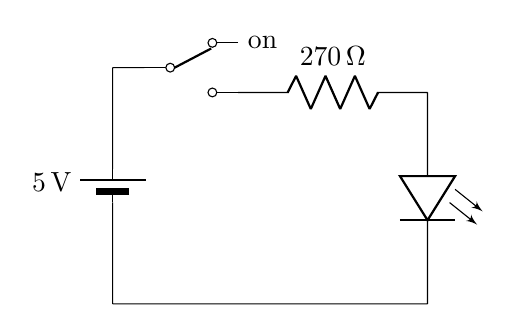
\begin{tikzpicture}
        \coordinate (as) at (4,3);
        \draw 
	(0, 3) to [battery2, l_=5<\volt>,] (0,0) 
	(1, 3) node[spdt] (Sw1) {}
	(0, 3) to [short] (Sw1.in)
		(Sw1.out 1) node[right] {on} 
	(Sw1.out 2) to [R,label=270<\ohm>] (as |- Sw1.out 2)
	(as |- Sw1.out 2) to [empty led] (4,0)
	(4,0) to (0,0);
      \end{tikzpicture}
      }
  \end{columns}
\end{frame}

\begin{frame}{Both Light Switches On}

  \begin{columns}
    \column{0.5\textwidth}
    \begin{itemize}
    \item
      Two switches in series (one after the other)
    \item
      You have to flick both to ``on'' for the lamp to work 
    \item
      Switch 1 AND Switch 2
    \end{itemize}

    \column{0.5\textwidth}
    \resizebox{\textwidth}{!}{
      \begin{tikzpicture}
        \coordinate (as) at (6,4);
        \draw 
	(0, 4) to [battery2, l_=5<\volt>,] (0,0) 
	(1, 4) node[spdt] (Sw1) {}
	(3,4) node[spdt, xscale=-1] (Sw2) {}
	(0, 4) to [short] (Sw1.in)
		(Sw1.out 1) node[right] {off}
	(Sw1.out 2) to (Sw2.out 2) 
	(Sw2.in) to [R,label=270<\ohm>] (as)
	(as) to [empty led] (6,0)
	(6,0) to (0,0);
      \end{tikzpicture}
      }
  \end{columns}
\end{frame}


\begin{frame}{Make Titles Informative.}

  You can create overlays\dots
  \begin{itemize}
  \item using the \texttt{pause} command:
    \begin{itemize}
    \item
      First item.
      \pause
    \item    
      Second item.
    \end{itemize}
  \item
    using overlay specifications:
    \begin{itemize}
    \item<3->
      First item.
    \item<4->
      Second item.
    \end{itemize}
  \item
    using the general \texttt{uncover} command:
    \begin{itemize}
      \uncover<5->{\item
        First item.}
      \uncover<6->{\item
        Second item.}
    \end{itemize}
  \end{itemize}
\end{frame}


\subsection{Second Subsection}

\begin{frame}{Make Titles Informative.}
\end{frame}

\begin{frame}{Make Titles Informative.}
\end{frame}



\section*{Summary}

\begin{frame}{Summary}

  % Keep the summary *very short*.
  \begin{itemize}
  \item
    The \alert{first main message} of your talk in one or two lines.
  \item
    The \alert{second main message} of your talk in one or two lines.
  \item
    Perhaps a \alert{third message}, but not more than that.
  \end{itemize}
  
  % The following outlook is optional.
  \vskip0pt plus.5fill
  \begin{itemize}
  \item
    Outlook
    \begin{itemize}
    \item
      Something you haven't solved.
    \item
      Something else you haven't solved.
    \end{itemize}
  \end{itemize}
\end{frame}


\end{document}


